% Author: Anachuri Nicolas Daniel
% Template for myself
 
\documentclass[11pt]{article}
\usepackage{indentfirst} 		% First line paragraph indentation
\usepackage{etoolbox} 			% Used for being able to utilise if statements in the language detection.
\setlength{\parskip}{\baselineskip}	% With this line, it is not needed the use of \\ at the end of each paragraph for spacing purposes


% ========================= VARIABLES TO MODIFY =================================

\def\LANGUAGE{EN} %EN, ES		%Language in which the document is going to be written.

\def\reportTile{Fisica Aplicada }			%Document's title
\def\subject{Trabajo Practico N.2}			%Subject

\def\writter{Anachuri Nicolas Daniel y Tito Benjamin }		%Author(s)


\def\leftUpperHeader{\subject}		%\subject
\def\rightUpperHeader{\leftmark}	%\leftmark for current section


% Do NOT modify anything from here until the beginning of the document.
%============================== DATA PROCESSING ============================
\ifdefstring{\LANGUAGE}{EN}
{

\def\course{1ro del Superior Informatica} %---------
\def\university{Escuela de Minas Dr. Horacio Carrillo} %------------
\def\pageCounterName{PAGE} 		% In the footer will be shown this... 
\def\pageSeparator{OUT OF} 		% ...text in addition of the page number.

}
{
\usepackage[utf8]{inputenc}		%Tildes en caso de no usar arch
\usepackage[spanish, es-tabla]{babel} 	%La opción es-tabla, hace que por defecto las tablas se llamen "Tabla", en vez de "Cuadro".
\def\course{1ro del Superior Informatica} %----------
\def\university{Escuela de Minas Dr. Horacio Carrillo}
\def\pageCounterName{PÁGINA}		%En el pie de página aparece este contenido más el número de página
\def\pageSeparator{DE} 			%DE, OUT OF

}


%===================== USEFUL VARIABLES  =============================
\def\imageSize{0.9}

%===================== PACKAGES TO USE  =============================
\usepackage{amsmath} 			% Allows me the use of matrix in math mode \setcounter{MaxMatrixCols}{20} 		% Increases the maximum number of columns in matrix from 10 to 20.
\usepackage{pdfpages} 			% Attach pdfs using \includepdf[pages=initial-final]{path.pdf}
\usepackage{lastpage}			% Used to reference the last page and include it in the footer.
\usepackage{xcolor}			% Change color of text and so on. \textcolor{color}{text} is the one I use the most.
\usepackage{placeins} 			% Allows the use of the command \FloatBarrier
\usepackage{setspace}			% Allows the use of the spacing environment to change the space between lines.
\usepackage{graphicx}			% Figures addition
\usepackage{wrapfig}
\usepackage{geometry}			% Changes the geometry of the pages
\usepackage[small, bf]{caption}		% Decreases the size of captions and turns them bold text.
\usepackage{subcaption}			% Include subfigures.
\usepackage{hyperref}			% Allows clickable references.
\hypersetup{colorlinks=true, allcolors=black} 	% Colors of links
\usepackage{pdflscape}			% Allows the use of the environment lscape for landscape pages

\usepackage{fancyhdr}			% Modify header and footer
\usepackage{bm}				% Allows to use bold text in math mode with \bm
\usepackage[makeroom]{cancel}		% Allows the use of \cancelto{}{} to cross out equations
\usepackage{titlesec}			% Change title format
\usepackage{multicol}
\usepackage{hyperref}

%========== CHANGE TITLE FORMAT  ======================
%\titleformat{\section}
%{\bfseries}	% format
%{\thesection}	% label
%{0.3cm}		% separation between label and body
%{}		% code preceding title body
%[]		% code following title body


%========== HEADER AND FOOTER CONFIGURATION ======================
\pagestyle{fancy}
% HEADER[EVEN PAGES]{ODD PAGES}
% Left header
\lhead[
	\scriptsize{\MakeUppercase{\leftUpperHeader}} % Even pages
]
{
	\scriptsize{\MakeUppercase{\leftUpperHeader}} % Odd pages
}

% Central header
\chead[]{}

% Right header
\rhead[
\scriptsize{\rightUpperHeader} % Even pages
]
{
\scriptsize{\rightUpperHeader} % Odd pages
}

\renewcommand{\headrulewidth}{0.8pt}	% Width of the header rule

% FOOTER[EVEN PAGES]{ODD PAGES}
% Left footer
\lfoot[]{}

% Central footer
\cfoot[
\tiny{\pageCounterName\space\thepage\space \pageSeparator\space\pageref{LastPage}} % Even pages
]
{
\tiny{\pageCounterName\space\thepage\space \pageSeparator\space\pageref{LastPage}} % Odd pages
}

% Right footer
\rfoot[]{}
\renewcommand{\footrulewidth}{0.8pt} %Width of the footer rule


%================================== USER OWN FUNCTIONS ===============================================
\newcommand{\PDEA}[1]{\cdot 10^{#1}} % Función para escribir más rápidamente multiplicaciones por potencias de 10. PDEA = Por Diez Elevado A

\usepackage{xargs}	%Permite manejar argumentos opcionales en los comandos creados por el usuario

%Incluir imágenes, la sintaxis es la siguiente:
%\IncludeImage{ruta}[escalado][pie figura][etiqueta], los corchetes son opcionales
\newcommandx*{\IncludeImage}[4][2=1, 3=, 4=]{
	%#1 es la ruta a la imagen
	%#2 es el escalado
	%#3 es el pie de figura
	%#4 es la etiqueta
	
	\begin{figure}[h!]
		\centering
		\includegraphics[width=#2\linewidth]{#1}
		%Si se especifica pie de figura...
		\ifblank{#3}{}{
			\caption{#3}	
		}
		%Si se especifica etiqueta...
		\ifblank{#4}{}{
			\label{#4}	
		}
	\end{figure}
	\FloatBarrier
}



%================================ DOCUMENT BEGINNING  =============================================
\begin{document}
%***************** TITLE PAGE (DO NOT MODIFY) ******************************
\begin{titlepage}
	\newgeometry{top=2cm, bottom=3.5cm}

	%Logos Escuela y universidad
	\def\logoSize{0.2}
	\begin{figure}
	\includegraphics[width=\logoSize\linewidth]{/home/nico/Descargas/minas.jpeg}
	\hfill
	\includegraphics[width=\logoSize\linewidth]{/home/nico/Descargas/unju.jpeg}
	\end{figure}


	%Espacio entre logos y título
	\vspace*{1.75cm}

	%Título con interlineado aumentado
	\begin{spacing}{2}
	\centering{
	\Huge{
		\textbf{\reportTile}
	}
	}
	\end{spacing}
	
	%Línea horizontal de la portada
	\hrule
	
	%Se baja al final de la hoja
	\vfill
	\begin{flushright}
	\LARGE{\writter}

	\vspace{2cm}
	
	\Large
	\subject\\
	\course\\
	\university
	
	\vspace{1cm}
	
	\today
	\end{flushright}
	
\end{titlepage}
	
\newgeometry{top=3cm, bottom=3cm}

\tableofcontents
%\cleardoublepage
\clearpage

\begin{multicols}{2}

\section{Descubrimiento de Titan}

\subsection{Expresen en 5 líneas cuál creen que es el motivo de este artículo}

Principalmente se centra en la divulgacion de informacion hacia la personas que no poseen los recursos para acceder a ellos y la difucion publica de conocimiento con el cual se pretende expandir las investigaciones de otros cientificos e investigadores gracias a la nueva informacion publicada. Se lo puede definir como una trabajo en conjunto entre varias ramas de le ciencia como la informatica , medicina , fisica , quimica , etc con el objetivo principal de rapidamente expandir los confines a los cuales la ciencia antes no era capaz de imaginar. 
   
\subsection{¿Qué se quiere expresar con la palabra “casualidad” en la primera oración?}
   
Se quiere expresar que el descubrimiento fue algo casual, es decir, que el des-cubrimiento de Titán no era el objetivo de Huygens en ese momento.

\subsection{¿Quiénes fueron John Herschel y su padre William Herschel?}
  
  Ambos fueron famosos astrónomos, William Herschel fue quién descubrió Uranoademás de otros cuerpos celestes. Por su parte, John Herschel, popularizó el usode la fecha juliana e inventó la cianotipia. \cite{william}\cite{john}
  
  \begin{wrapfigure}{0.6\linewidth}
  
  \centering
  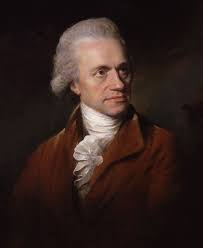
\includegraphics[width=0.6\linewidth]{william.jpeg}
  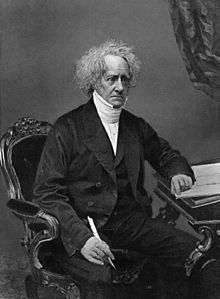
\includegraphics[width=0.6\linewidth]{john.jpg}
  \caption{William Herschel y John Herschel}
  %\label{fig:etiqueta}
  
\end{wrapfigure}


\subsection{¿A qué capítulo de la física, a su entender refiere la presente nota?}
\label{sec:1}

\textbf{Fisica Moderna: Fisica Relativa}: es la rama encargada de analizar los movimientos de los cuerpos de acuerdo a la relacion que se establece entre el espacio y el tiempo, tomando como consideracion que la luz es la unica constante en el universo. Se basa en la Teoria de la Relatividad de Einstein. \cite{fisica}


\textbf{Astrofisica}: se encarga de estudiar el movimiento , estructura , composicion y evolucion de los cuerpos celestes. \cite{fisica}

\section{Horizonte de Eventos}
 \begin{wrapfigure}{0.6\linewidth}
  
  \centering
  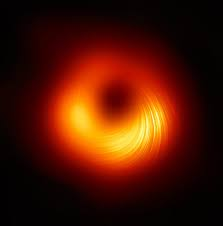
\includegraphics[width=0.6\linewidth]{hole.jpeg}
   \caption{Horizonte de Evento de un Agujero Negro}
  %\label{fig:etiqueta}
  
\end{wrapfigure}

 
\subsection{El artículo habla de luz polarizada ¿está explicado en el mismo el conceptode luz polarizada?}

Sí, está explicado el concepto de luz polarizada en el artículo.

\subsection{Cuando habla de chorros de partículas, ¿a qué partículas se refiere?S}

 Se refiere a partículas de materia circundantes que logran escapar momentosantes de quedar atrapadas dentro del agujero negro.

\subsection{¿Qué distancia representa (en Km) 55 millones de años luz?}

  Si un año luz equivale a 9,46×1012(9.460.730.472.580,8) Km, entonces 55millones de años luz equivale a:  \cite{luz}

\begin{wrapfigure}{0.7\linewidth}
  
  \centering
  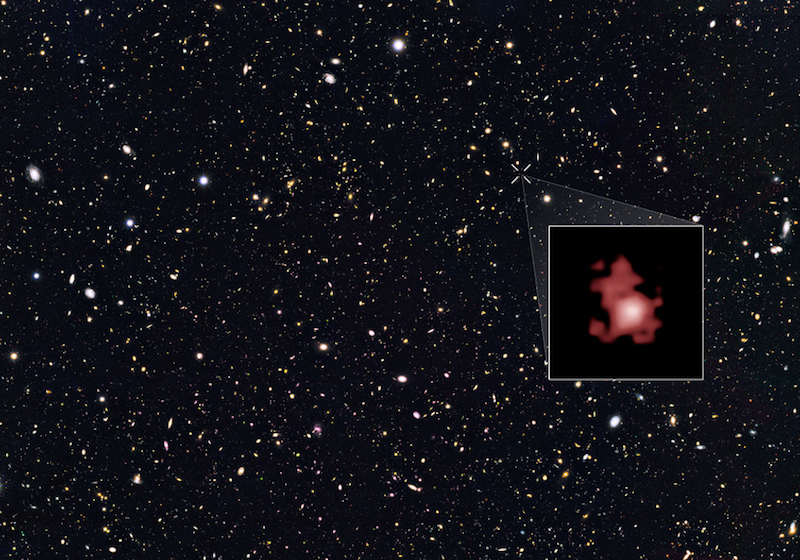
\includegraphics[width=0.6\linewidth]{year.png}
  \caption{Galaxia mas lejana captada por el Telescopio Hubble}
  %\label{fig:etiqueta}
  
\end{wrapfigure}

\subsection{Busque un modelo teórico que explique el comportamiento del gas magnetizado.“}

  “La presencia de gas magnetizado entre galaxias o estrellas de una misma galaxiapodría explicarse por intensos campos magnéticos generados probablemente en elUniverso poco después de que se produjera el "Big Bang", según las conclusionesde un equipo internacional de astrofísicos del CNRS.”"La interacción entre energía turbulenta, una suerte de energía cinética generadapor la turbulencia, y campo magnético puede amplificar un campo inicialmentedébil y darle fuerza", reiteran los científicos, que con ese acercamiento profundizanen la manera en que las líneas de los campos magnéticos interactúan con losbloques turbulentos.\cite{gases}

\subsection{¿Qué relación cree usted que hay en ambos artículos?}
  
  La relación que hay ambos artículos es que ambos descubrimientos están dentro del campo de estudio de la astrofísica\href{sec:1} , que es el desarrollo y estudio de la física aplicada la astronomía y la Fisica Relativa\href{sec:1}.
  
  
\begin{thebibliography}{100}
    
\bibitem{luz}   NASA (The National Aeronautics and Space Administration) https://spaceplace.nasa.gov/light-year/en/
  
\bibitem{john} The Times https://en.wikipedia.org/wiki/John-Herschel
   
\bibitem{william} The Times https://en.wikipedia.org/wiki/William-Herschel 
  
\bibitem{fisica} Burkhardt, H. (1987). System physics: A uniform approach to the branches of classical physics. American Journal of Physics, 55, 344. https://aapt.scitation.org/doi/10.1119/1.15167
  
\bibitem{gases}   A.M. Ingham and J.K. Gilbert, Int. J. Phys. Ed. 13, 193 (1991).  http://www.scielo.br/scielo.php?script=sci-arttext&pid=S1806-11172005000300020


\end{multicols}





\end{document}

